
\documentclass{article}
\usepackage[utf8]{inputenc}
\usepackage{geometry}
    \geometry{
    left=0.5in,
    top=0.5in,
    right=0.5in,
    bottom=0.75in
    }
\usepackage{enumitem} % https://latex.org/forum/viewtopic.php?t=28712
\usepackage{mdframed}
\usepackage{listings}
\usepackage{graphicx}
\graphicspath{ {../../common_images/} {./images/} {.} }
\usepackage{hyperref}
\hypersetup{colorlinks,urlcolor=blue}

\usepackage{soul} % strikethrough with \st{}

\usepackage{amsmath}  % for the recurrences with multiple cases

\usepackage{xcolor}

\definecolor{codegreen}{rgb}{0,0.6,0}
\definecolor{codegray}{rgb}{0.5,0.5,0.5}
\definecolor{codepurple}{rgb}{0.58,0,0.82}
\definecolor{backcolour}{rgb}{0.95,0.95,0.92}

\lstdefinestyle{mystyle}{
    backgroundcolor=\color{backcolour},   
    commentstyle=\color{codegreen},
    keywordstyle=\color{magenta},
    numberstyle=\tiny\color{codegray},
    stringstyle=\color{codepurple},
    basicstyle=\ttfamily\footnotesize,
    breakatwhitespace=false,         
    breaklines=true,                 
    captionpos=b,                    
    keepspaces=true,                 
    numbers=left,                    
    numbersep=5pt,                  
    showspaces=false,                
    showstringspaces=false,
    showtabs=false,                  
    tabsize=2
}

% \lstdefinestyle{mystyle}{
%     basicstyle=\ttfamily\footnotesize,
%     breakatwhitespace=false,         
%     breaklines=true,                 
%     captionpos=b,                    
%     keepspaces=true,                 
%     numbers=left,                    
%     numbersep=5pt,                  
%     showspaces=false,                
%     showstringspaces=false
% }
 
\lstset{style=mystyle}

% Source: https://tex.stackexchange.com/questions/30720/footnote-without-a-marker
\newcommand\blfootnote[1]{%
  \begingroup
  \renewcommand\thefootnote{}\footnote{#1}%
  \addtocounter{footnote}{-1}%
  \endgroup
}

% https://www.overleaf.com/learn/latex/Questions/How_do_I_tab_(indent)_a_paragraph_in_LaTeX%3F
\usepackage{indentfirst}

\title{ECS 32B: Conceptual Homework \#2}
\author{Instructor: Aaron Kaloti}
\date{Summer Session \#2 2020\blfootnote{This content is protected and may not be shared, uploaded, or distributed.}}

\begin{document}

\maketitle

% \tableofcontents

\section{Changelog}

You should always refer to the latest version of this document.

\begin{itemize}[itemsep=0mm, parsep=0pt]
\item v.1: Initial version.
\item v.2: Added a note about a LaTeX directive called \lstinline{setcounter}.
\item v.3: Replaced mention of \lstinline{high} with \lstinline{last} in one of the binary search problems. Added a note about code listings for the more time-efficient queue question.
\end{itemize}

\section{Grading}

\begin{itemize}[itemsep=0mm, parsep=0pt]
\item \textbf{Due date}: the night of Thursday, 09/03. (Due to the ``grace period'', Gradescope will say 12:30 AM on Friday, 09/04.)
\item A subset of the problems will be graded for correctness. The rest will be graded on completion.
\end{itemize}

\section{Submission Requirements}

\begin{itemize}[itemsep=0mm, parsep=0pt]
\item Your submission must be typed with LaTeX. \textbf{Handwritten/scanned solutions, or solutions not typed with LaTeX, will earn no credit.}
    \begin{itemize}[itemsep=0mm, parsep=0pt]
    \item You should avoid doing this assignment at the last minute, because it will take a bit of time to get used to LaTeX and to type your answers up into a LaTeX document.
    \end{itemize}
\item Your submission must consist of one file, the PDF generated by your LaTeX file (\lstinline{hw2_answers.pdf}). Since Gradescope does not let you submit files that are neither PDFs nor images, I will not have you submit the \lstinline{.tex} file. However, if it is clear that your submission was not made with LaTeX, we may email you to ask that you send us your \lstinline{.tex} file, and if you cannot (i.e. if it turns out that your PDF was in fact not created with LaTeX), you will get a zero on this assignment.
\item You may be penalized if, when submitting on Gradescope, you mark the wrong page for a given homework problem, because dealing with this slows down grading. In the middle of the 08/06 lecture, I talk about how to mark the pages of your submission on Gradescope, starting at around 1:03:55 in the video.
\item When using LaTeX, you should make use of the math notation/mode where sensible. (The math mode refers to when you put mathematical equations, etc. between dollar signs so that LaTex makes them look nice.) Repeated failures to do this, to the point that the purpose of using LaTeX is defeated or the readability of your answers is impeded, may result in a penalty on this assignment.
\end{itemize}

\section{Regarding Collaboration}

\begin{itemize}[itemsep=0mm, parsep=0pt]
\item You may not copy answers from any sources, including online sources such as Chegg, StackOverflow, or any solutions manual of any textbook.
\item You may partner with \textbf{\textit{at most one}} other student on this assignment. In other words, you can work in \textit{pairs}. You do not have to partner with anyone. (In fact, I think it is better that you do not.) If you partner with someone, it must be a committed partnership; that is, you two will have the same submission, and you must mark on Gradescope that you have partnered for this assignment by following the directions \href{https://www.youtube.com/watch?v=rue7p_kATLA}{here}.
\item If students that were not in the same pair seem to have excessively similar answers, they will be reported to the OSSJA for suspicion of academic misconduct. Do not copy answers from (or share answers with) any student who you are not partnered with.
\end{itemize}

\section{Identification}

Enter the members of your pair. (You can partner with at most one other student.) If you are not partnered with anyone, then leave the second box empty. You can remove the use of \lstinline{\vspace} in the \lstinline{.tex} file.

Pair member \#1:

\begin{mdframed}
\vspace{3em}
%% TODO
\end{mdframed}

Pair member \#2:

\begin{mdframed}
\vspace{3em}
%% TODO
\end{mdframed}

\section{Problems}

Unless explicitly specified, you do not need to justify your answer. Place your answer into the answer boxes; you can remove the use of \lstinline{\vspace} in the answer boxes in the \lstinline{.tex} file. If you are using your own LaTeX template, you may find the \lstinline{setcounter} directive useful; it lets you set the number of the next section, and you can read more \href{https://tex.stackexchange.com/questions/200437/numbering-sections-subsections-etc-manually}{here}.

\subsection{Linked List Indexing}

Explain why linked lists do not support constant time indexing.

\begin{mdframed}
\vspace{3em}
%% TODO
\end{mdframed}

\subsection{Unordered List \lstinline{add()}}

Consider the implementation of \lstinline{add()} for the linked list implementation of an unordered list on slide \#30 of the linear data structures slide deck. Could we flip the order of the lines \lstinline{temp.setNext(self.head)} and \lstinline{self.head = temp}? If \textit{not}, explain.

\begin{mdframed}
\vspace{3em}
%% TODO
\end{mdframed}

\subsection{Stack-Less Balanced Symbols}

\subsubsection{Balanced Parentheses}

Recall the balanced parentheses example from the lecture on stacks (and from your primary textbook). Could we have replaced the stack with a single integer variable instead? If so, explain how we would adjust the approach to the balanced parentheses problem (i.e. when and how would the integer variable change? how can it be used to detect that the given string of parentheses is unbalanced?). If not, explain why.

\begin{mdframed}
\vspace{3em}
%% TODO
\end{mdframed}

\subsubsection{Balanced Symbols}

Repeat the previous problem, except for the more general balanced symbols example (that you were supposed to read about in section 4.7 of the primary textbook) instead.

\begin{mdframed}
\vspace{3em}
%% TODO
\end{mdframed}

\subsection{Binary Search on an Ordered List}

When we talked about ordered lists during lecture, we added a small speed-up to the \lstinline{search()} method that did not affect the worst-case time complexity. Why did we not use binary search? Should we have? If we had implemented the ordered list with a Python list instead of a linked list, could we have used binary search there instead/too? How, if at all, would that have improved the worst-case time complexity of \lstinline{search()}?

\begin{mdframed}
\vspace{3em}
%% TODO
\end{mdframed}

\subsection{Binary Search Midpoint Calculation}

In our Python implementation of binary search, why do we not calculate \lstinline{midpoint} by using the formula \lstinline{midpoint = last // 2}.

\begin{mdframed}
\vspace{3em}
%% TODO
\end{mdframed}

\subsection{Unordered List \lstinline{remove()}}

\subsubsection{Worst-Case Time Complexity}

As stated on slide \#40, if we use a Python list as an unordered list (think of just a normal Python list of integers, with nothing special about it), \lstinline{remove(item)} takes linear time, \textit{regardless} of the location of \lstinline{item}. Why does the location of \lstinline{item} not matter? Why would removing the element at the front of the unordered list (again, represented as a Python list) take about as long (i.e. linear time) as removing the element at the end?

\begin{mdframed}
\vspace{3em}
%% TODO
\end{mdframed}

\subsubsection{Removing the Last Node}

Explain how the \lstinline{remove()} method for the linked list representation of an unordered list (see slide \#37 of the linear data structures slide deck) works if the node-to-remove is the last node in the linked list.

\begin{mdframed}
\vspace{3em}
%% TODO
\end{mdframed}

\subsubsection{Removing the Only Node}

Consider the same implementation of \lstinline{remove()} that was considered in the previous question. Explain how that implementation works if the node-to-remove is the \textit{only node} in the linked list.

\begin{mdframed}
\vspace{3em}
%% TODO
\end{mdframed}

\subsection{A More Time-Efficient Queue}

Recall that for the implementation of a queue that we examined during lecture, \lstinline{enqueue()} runs in linear time in the worst case. Suppose we wanted to implement a queue (i.e. a queue class) such that \textit{all} of its operations, including \lstinline{enqueue()}, take constant time, and suppose that we were assured that never more than $100$ elements would be inserted into an instance of this queue \textit{ever}. For example, we could see that $50$ elements are inserted into an instance of the queue, followed by $4$ pops, and then followed by $50$ more insertions, but after this, we are assured that there won't be a $101$st insert. How can we implement such a queue that has constant time operations? You should explain your approach and explain how each of \lstinline{enqueue()}, \lstinline{dequeue()}, and \lstinline{size()} would be implemented and how they each take constant time. Explain how your approach might work in a small hypothetical scenario, e.g. a mix of 1-2 calls to \lstinline{enqueue()} and 1-2 calls to \lstinline{dequeue()}.

\textit{Hint}: Use a Python list as the underlying implementation. Take advantage of a concept called ``lazy deletion''. To ``lazily delete'' from a Python list is to ``trick'' your code into thinking that an element was deleted (usually from the front or back) of the list by changing some variables in your code that keep track of where the start or end of the Python list is.

\begin{mdframed}
\vspace{3em}
%% TODO
\end{mdframed}

If you want, you could provide code for this question, using the LaTeX code listings feature, as demonstrated below. See the \lstinline{.tex} file for how it's done. \textcolor{red}{Please erase, or comment out, this part if you don't use it.}

\begin{lstlisting}[language=Python]
print("Hello world!")
\end{lstlisting}

\subsection{Full Binary Trees vs. Complete Binary Trees}

A full binary tree is a binary tree in which each node that is not a leaf has two children. Below is an example.

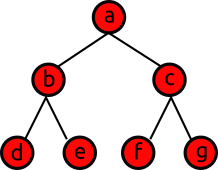
\includegraphics{full_binary_tree}

A complete binary tree is a binary tree in which every level, except possibly the last (which has all of its node shifted as far left as possible), is filled. Give \textbf{\textit{and explain}} an example that shows that a full binary tree is not always complete. (By ``explain'', I mean that you should explain how your example shows what you want it to show.) If you wish, you can upload an image, even if the image is handwritten, using \lstinline{includegraphics}; see how it's used in the LaTeX file to include the full binary tree and complete binary tree images, and note that the file extension must be omitted.)

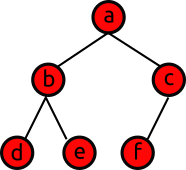
\includegraphics{complete_binary_tree}

\begin{mdframed}
\vspace{3em}
%% TODO
\end{mdframed}

% \begin{center}
% 
\includegraphics[scale=0.4]{UCD_CS_Logo}
% \end{center}

\end{document}
